% Author: Joshua Carey

%
\let\textcircled=\pgftextcircled
\chapter{Methodology}
% \label{chap:aims_and_opjectives}

% \initial{T}his section will investigate the approach taken to create an autonomous kite-powered vessel.
% - We need a physics engine
% -we need to model a boat so that it behaves with realistic movements
% - need to be able to run machine learning in the physics simulations

% \initial{T}he future of autonomous navigation in maritime settings is not limited to large vessels plying the world's oceans; smaller, nimble crafts, harnessing natural forces such as wind, present their own set of challenges and opportunities. Imagine a vessel, propelled not just by the currents below, but by the gusts above, using a kite to harness the power of the wind. This not only promises sustainable navigation but also offers a glimpse into the intricate dance between machine intelligence, physics, and nature's unpredictability. This project dives deep into simulating such a system— a kite-powered boat that autonomously navigates its environment. This methodology section elucidates the steps taken to bridge the gap between vision and virtual reality.

\initial{T}his section will investigate the approach taken to create an autonomously controlled kiteboat in a simulation. As discussed in section 2.2 Reinforcement Learning (RL) is an appropriate type of ai for the control of a kiteboat. RL works on a trail and error approach and its core loop is shown in figure LABLE.

\begin{figure}[h]
    \centering
    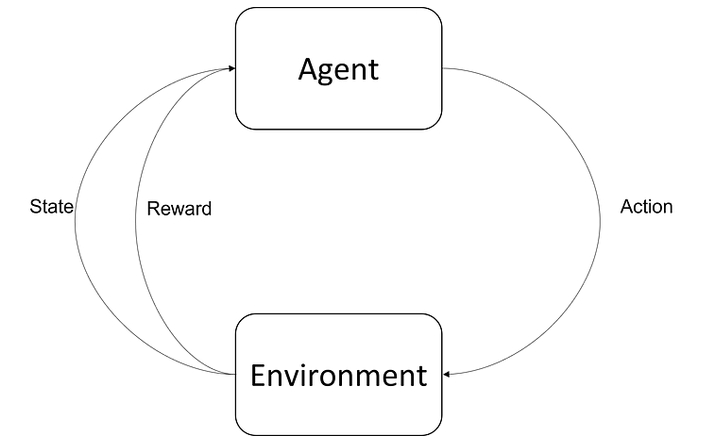
\includegraphics[width=0.5\textwidth]{Images/RL_Loop.png}
    \caption{The RL Loop}
\label{RL_loop}
\end{figure}


\section{The Environment}

The first step to this process if to create the environment, which the agent will use to train. In this case that will need to look something like a sailing game; it will have some form of water, a boat, a kite and a course. 
For any machine learning endeavor, especially one with such intricate physical dynamics, the choice of simulation environment is paramount. Not only does it provide the playground for our AI agent to learn and make mistakes safely, but it also serves as a litmus test for the robustness and realism of the designed model.

Given the myriad of choices available, the Unity game engine emerged as the most suitable platform. Beyond its reputation in gaming, 
The inherent support for mesh bodies, colliders, and a variety of joints made it an attractive option for simulating the kite-boat system, which comprised a complex dance of forces, and counterforces.
Unity is recognized for its potent physics engine, however for this project the use of Unity's physics engine will be kept to a minimum. Unity will be used primarily for its visual capabilities and the ability to run machine learning simulations. 

Central to our simulation is the depiction of water, the medium in which our boat will navigate. Here, the Unity HDRP Water System 16.0.3 [cite] came to the rescue. Bundled with Unity 2023.2.0b9 [cite], this water system provides a realistic representation of water with its undulating waves, refractions, and reflections. 
The alternative option to using Unity's water system was to model an entire particle fluid simulation, this would have had its advantages, however it would have been a lot more computationally expensive and would have taken a lot longer to implement. As this project was primarily focused on creating a RL algorithm for controlling a kiteboat it was decided that the Unity water system would be sufficient for this project.  

The boat part of the kiteboat had two main component scripts, the buoyancy and the rudder, allowing the boat to float and be steered. The implementation of Buoyancy and the rudder are discussed in more detail in section$~$\ref{sec:Buoyancy} and$~$\ref{sec:Rudder} respectively. 

Several assumptions were made before modeling the boat, these were primarily made to save time on the implementation and were deemed to have insignificant effects on the overall performance of the boat. These assumptions were:
\begin{itemize}
    \item The Archimedes force is uniform across all submerged sections of the boat.
    \item The rudder forces of lift and drag could be aproximated to a torque applied to the boat.
    \item Once the boat is moving at a speed greater than 0.25m/s the lift and drag forces of the keel are equal to the downwind component of the kite's resultant force- essentially providing a non'slip condition.
\end{itemize}
\subsection{Buoyancy}\label{sec:Buoyancy}
Buoyancy, the force that allows ships to float, was the first physical property to be addressed. Rooted in Archimedes' Principle, it dictates that the buoyant force exerted on a submerged body is equivalent to the weight of the fluid displaced by that body. In our Unity environment, the boat's hull, represented as a `mesh' with an associated `mesh collider', was divided into many small triangles or Voxels. These Voxels became the fundamental units for calculating buoyancy, allowing for a granular and realistic representation of the boat's interaction with water. This was achieved by first calculating the total Archimedes force (AF) of the entire boat using equation$~$\ref{archimedes}, followed by a local AF at each Voxel. The water level, y component, was then computed at each voxel's (x,z) coordinates to determine if it was above or below the surface. If below the surface the component of the AF was applied vertically at each voxel. This implementation can be viewed in the buoy.cs script in the project REF IN APENDIX.

\begin{equation}
    F_B = \rho_{w}gV
    \label{archimedes}
\end{equation}


\subsection{Rudder}\label{sec:Rudder}
While buoyancy ensures our boat doesn't sink, it's the rudder that grants it direction. The Rudder.cs script handles the implementation of the rudder and the keel. Several assumptions were made 
% The rudder was created as a rigid body and modeled as a simple symmetric foil using the force diagram in figure$~$\ref{rudderForce}. The lift and drag forces were calculated using equation$~$\ref{lift} and$~$\ref{drag}, where ${C_l}$ is the lift coefficient, ${C_d}$ is the drag coefficient, A is the sing surface area, V is the velocity of the water and ${\rho}$ is the density of the water.


% \begin{equation}
%     L = {C_l}A\rho\frac{V^2}{2}
%     \label{lift}
% \end{equation}
% \begin{equation}
%     D = {C_d}A\rho\frac{V^2}{2}
%     \label{drag}
% \end{equation}
 
% \begin{figure}
%     \centering
%     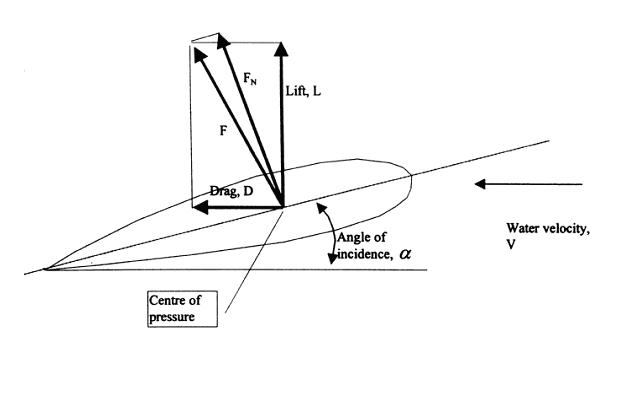
\includegraphics{chapters/chapter04/rudder.JPG}
%     \caption{Force Diagram of a boat rudder}\label{rudderForce}
% \end{figure}



\subsection{Course Generation}

\subsection{Mark Roundings}

\section{MLAgents}

\section{The Environment Structure}
Keep alive problem.

Diverse conditions

ciriculum style learning

\section{Initial Training}

\section{Optimization}

\subsection{Blue Crystal HPC}

The Blue Crystal HPC, operated by the University of Bristol, offers significant computational resources tailored for intensive tasks such as machine learning simulations, like.


To utilize Blue Crystal for MLAgents simulations, the following steps were undertaken:

\begin{itemize}
    \item \textbf{Access and Security:} Gained access to the university's HPC and set up SSH keys for secure communication.
    \item \textbf{File Preparation:} Built the .x86\_64 Unity build file and uploaded it, along with the necessary config file, to Google Drive.
    \item \textbf{Automation with Shell Script:} Developed a shell script to automate the process. This script:
    \begin{itemize}
        \item Retrieves the build files from Google Drive.
        \item Sets up a virtual environment on Blue Crystal.
        \item Installs the ML-Agents toolkit.
        \item Initiates the simulation.
        \item Upon completion, uploads the results back to Google Drive\textsuperscript{3}.
    \end{itemize}
\end{itemize}

Useful commands for working with Blue Crystal:

\begin{itemize}
    \item \textbf{sbatch:} Submits a job to the queue.
    \item \textbf{sacct:} Checks the status of a job.
    \item \textbf{scancel:} Cancels a job.
\end{itemize}

Parallelization and Optimization:

Initially, a single node on Blue Crystal was employed to run the simulation. This node with 28 CPUs was responsible for both hosting the environment and executing the model. However, Blue Crystal's architecture allows for more advanced parallelization strategies. Distributing the simulation across multiple nodes can enhance efficiency. Additionally, offloading the ML-Agents toolkit to a GPU core can further accelerate the learning process.

However, it's worth noting that the demand for GPUs on Blue Crystal is high. For tasks that don't necessitate the power of GPUs, relying on CPUs, even if they take longer, is a practical choice given the limited GPU availability.

%=======
\label{sec:sec01}





%=========================================================